% Versão de publicação. Gerado por experimentos/conteudo/graficos_publicacao.py.
% Requer \usepackage{graphicx}. Figuras já estão no tamanho de impressão (7,0 ou 3,5/4,6 pol.).
% Ajuste o caminho com \graphicspath{{entrega/graficos_publicacao/}}.

\begin{figure*}[htbp]
\centering
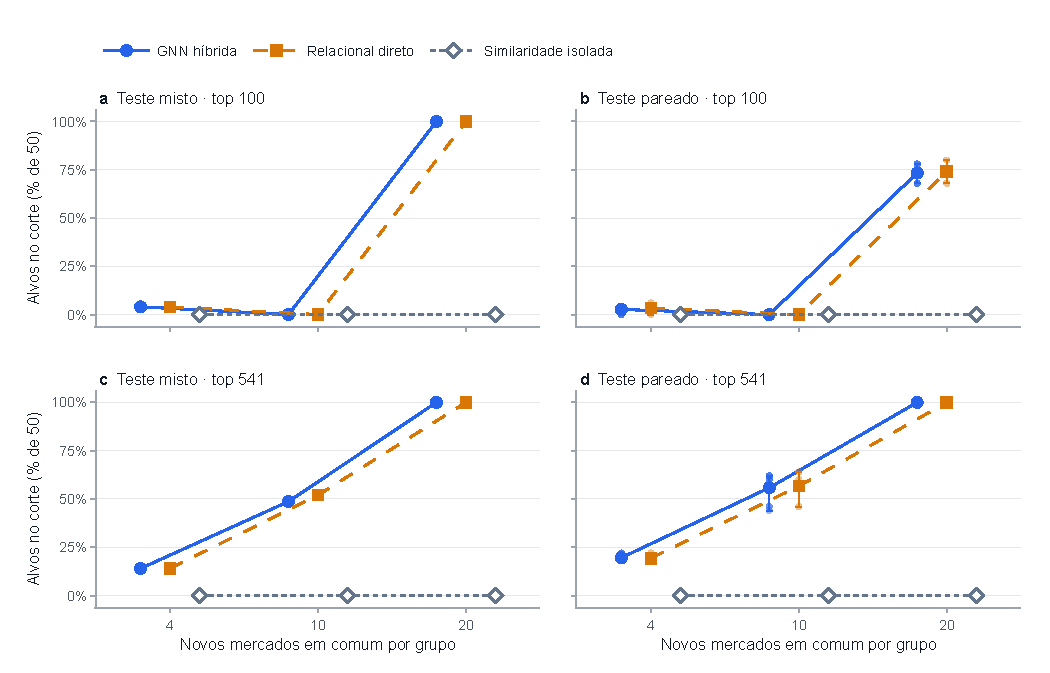
\includegraphics[width=\textwidth]{G1_recuperacao_intensidade.pdf}
\caption{Recuperação dos alvos artificiais por intensidade. Percentual dos 50 alvos no top 100 (a, b) e no top 541 (c, d). Pontos claros: cada ranking (misto: 3 seeds; pareado: 3 sorteios $\times$ 3 seeds; o relacional é determinístico e tem 1 ranking por sorteio). Marcador cheio: média entre rankings; barra: mínimo e máximo observados entre rankings (dispersão empírica, não intervalo de confiança). Os métodos são deslocados horizontalmente para não se sobreporem.}
\label{fig:g1}
\end{figure*}

\begin{figure}[htbp]
\centering
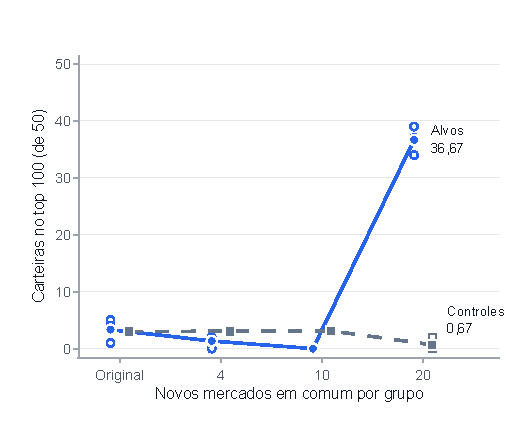
\includegraphics[width=\columnwidth]{G2_alvos_vs_controles.pdf}
\caption{Alvos e controles no teste pareado (GNN híbrida): carteiras no top 100, de 50 em cada categoria. Marcadores vazados: cada um dos 3 sorteios (média das 3 seeds, que coincidem); linha: média dos sorteios. Controles têm o mesmo grau inicial do alvo e ligações intactas.}
\label{fig:g2}
\end{figure}

\begin{figure*}[htbp]
\centering
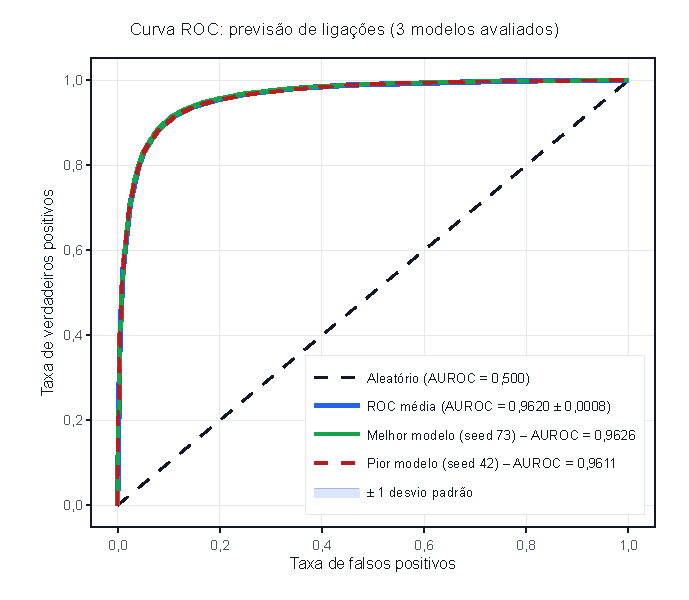
\includegraphics[width=4.6in]{G3_curva_roc.pdf}
\caption{Curva ROC da previsão de ligações no teste reservado (22.907 positivos e 22.907 negativos por modelo, grafo de contexto). Cinza: os 3 modelos (seeds 42, 73 e 2026), que compartilham a mesma divisão e os mesmos pares de teste e diferem só na inicialização e no treino; a variação mede, portanto, a sensibilidade à seed. Azul: média vertical das curvas interpoladas numa grade comum de FPR, com faixa de $\pm$1 desvio padrão amostral (n = 3, limitada a [0, 1]); a faixa é quase imperceptível porque o maior DP da TPR entre seeds é 0,011. A legenda traz o AUROC médio entre modelos $\pm$ DP; a área sob a curva média interpolada é 0,9620. Melhor e pior modelo pelo AUROC oficial (diferença de 0,0015). Curvas empíricas em degraus. A região até 10\% de falsos positivos está ampliada na figura de detalhe (G3\_curva\_roc\_detalhe, suplemento).}
\label{fig:g3}
\end{figure*}

\begin{figure*}[htbp]
\centering
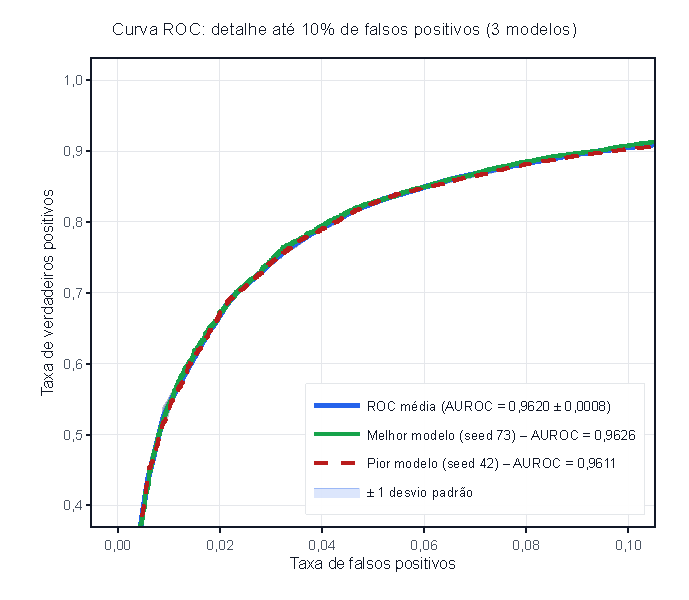
\includegraphics[width=4.6in]{G3_curva_roc_detalhe.pdf}
\caption{Detalhe da curva ROC (G3) na região de até 10\% de falsos positivos (TPR de 0,4 a 1,0), com os mesmos elementos e escala linear. Os eixos foram recortados para ampliar a região: as curvas continuam até FPR = 1.}
\label{fig:g3-detalhe}
\end{figure*}

\begin{figure*}[htbp]
\centering
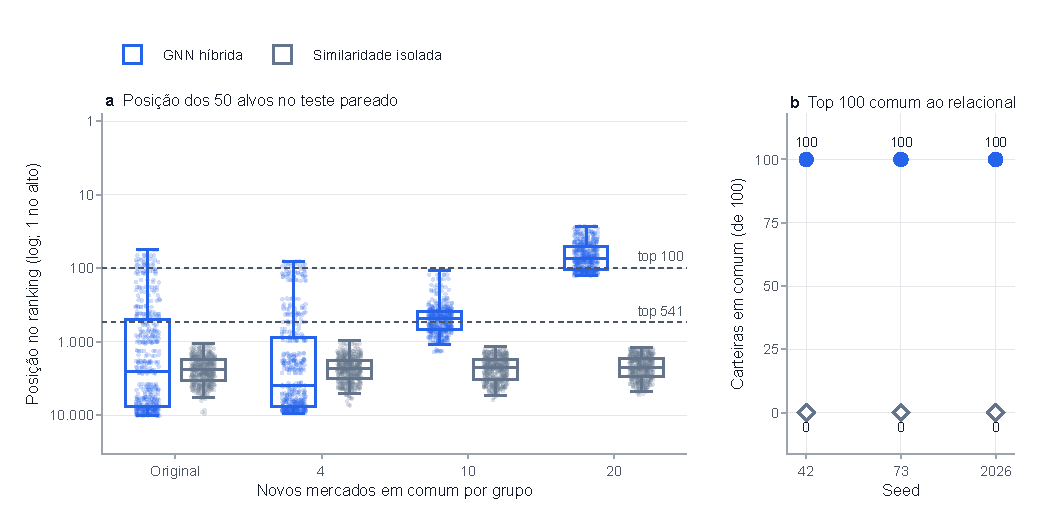
\includegraphics[width=\textwidth]{G4_comparacao_gnns.pdf}
\caption{GNN híbrida versus similaridade isolada: mesmos embeddings e mesmo treino (mesma AUROC); só muda o score de carteira. (a) Todas as posições dos 50 alvos em cada ranking do teste pareado (3 sorteios $\times$ 3 seeds = 450 por caixa); caixa: quartis e mediana; bigodes: 1,5 $\times$ IQR; todos os pontos são mostrados. (b) Carteiras do top 100 de cada GNN presentes também no top 100 do relacional no dia real.}
\label{fig:g4}
\end{figure*}

\begin{figure*}[htbp]
\centering
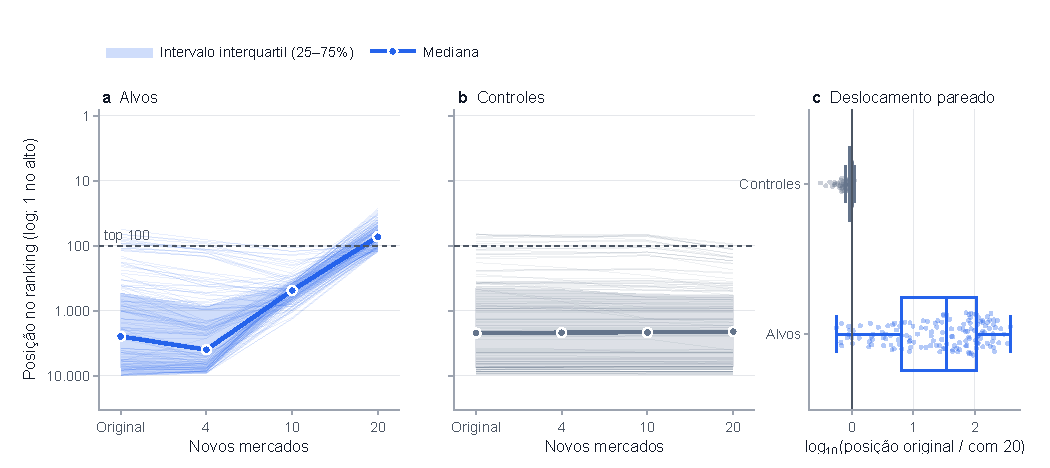
\includegraphics[width=\textwidth]{G5_trajetorias_pareadas.pdf}
\caption{Trajetórias pareadas no teste pareado (GNN híbrida, seed 42, 3 sorteios: 150 alvos e 150 controles). (a, b) Linhas finas: cada carteira; faixa: intervalo interquartil entre carteiras; linha forte: mediana. (c) Deslocamento de cada carteira entre o grafo original e 20 mercados, em log10 da razão das posições (positivo = subiu); caixa: quartis, bigodes 1,5 $\times$ IQR, todos os pontos mostrados.}
\label{fig:g5}
\end{figure*}

\begin{figure*}[htbp]
\centering
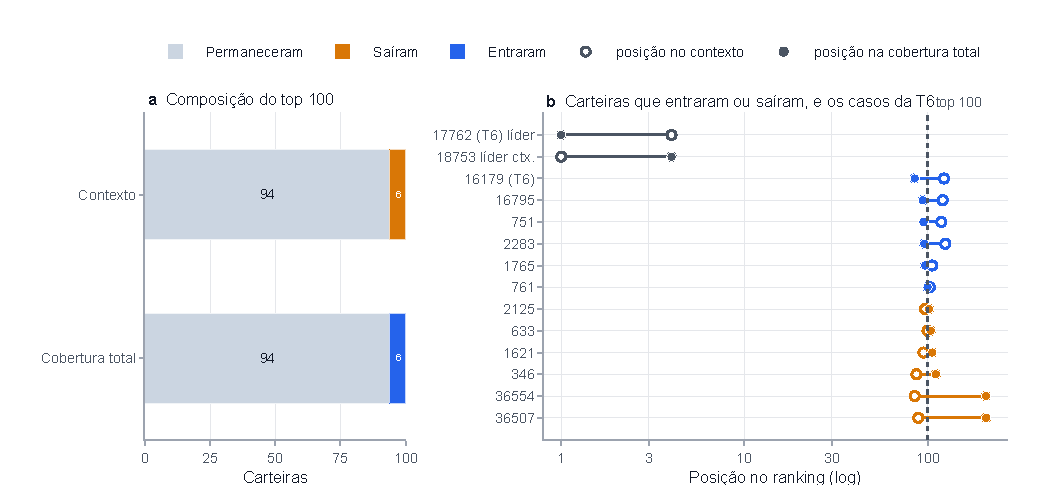
\includegraphics[width=\textwidth]{G6_entradas_saidas_top100.pdf}
\caption{Top 100 do dia real com as ligações de contexto e com a cobertura total (GNN híbrida, seed 42). (a) 94 carteiras permaneceram; 6 saíram e 6 entraram. (b) Posição no contexto (vazado) e na cobertura total (cheio) das carteiras que entraram ou saíram, dos casos da T6 e dos líderes. Não há fluxo entre carteiras: cada linha é a mesma carteira.}
\label{fig:g6}
\end{figure*}

\begin{figure*}[htbp]
\centering
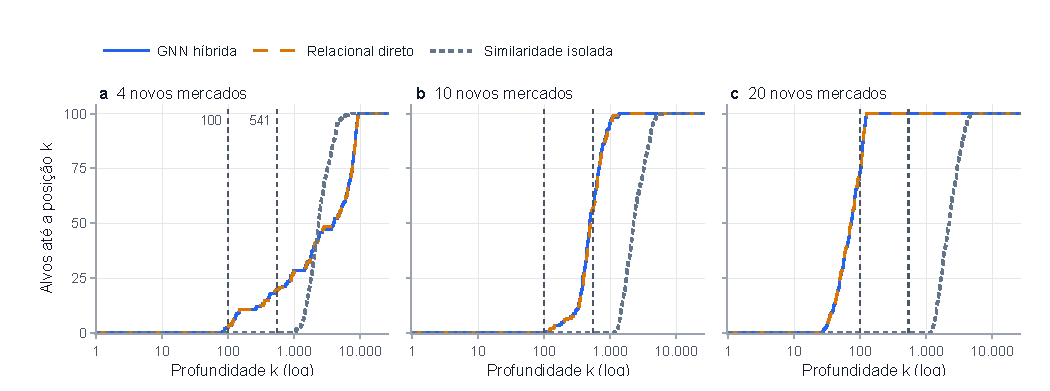
\includegraphics[width=\textwidth]{S1_recuperacao_acumulada.pdf}
\caption{Recuperação acumulada pela profundidade do ranking no teste pareado: percentual dos 50 alvos até a posição k, média dos rankings (3 sorteios $\times$ 3 seeds; 3 rankings no relacional), em degraus exatos. Linhas pontilhadas: cortes 100 e 541. O relacional (tracejado) quase coincide com a GNN híbrida.}
\label{fig:s1}
\end{figure*}

\begin{figure*}[htbp]
\centering
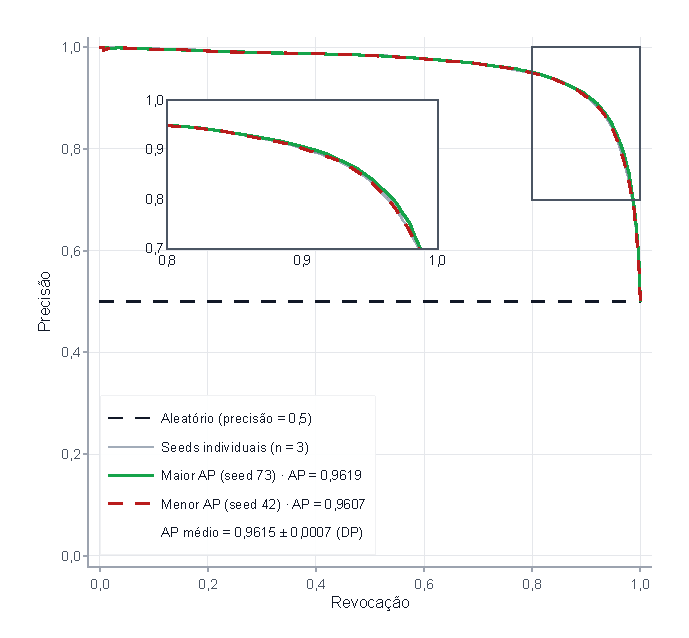
\includegraphics[width=4.6in]{S2_precisao_revocacao.pdf}
\caption{Curva precisão–revocação das ligações reservadas, por seed (mesmos pares de teste nas três). AP é a soma por limiar de (R\_n − R\_\{n−1\}) · P\_n, a mesma definição da T2, não a área trapezoidal. Não se desenha uma curva média: a média vertical de precisões não corresponde a nenhum AP. Linha tracejada: precisão de um classificador aleatório com negativos 1:1. O quadro mostra a região ampliada.}
\label{fig:s2}
\end{figure*}

\begin{figure*}[htbp]
\centering
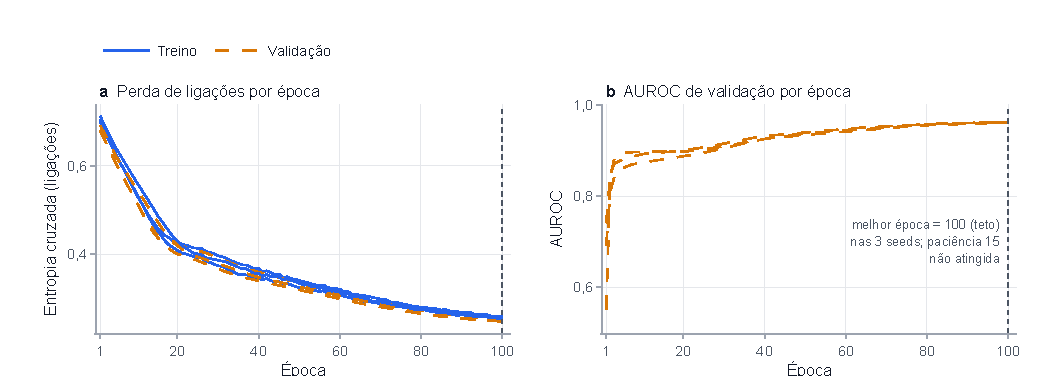
\includegraphics[width=\textwidth]{S3_perdas_treino.pdf}
\caption{Treino da GNN híbrida, uma linha por seed (3), sem suavização. (a) Perda de ligações no treino (contínua; sem o termo de contraste de peso 0,1) e na validação (tracejada). (b) AUROC de validação. A melhor época foi a última (100) nas três seeds: a parada antecipada (paciência 15) não foi atingida, e a perda de validação ainda caía.}
\label{fig:s3}
\end{figure*}

\begin{figure*}[htbp]
\centering
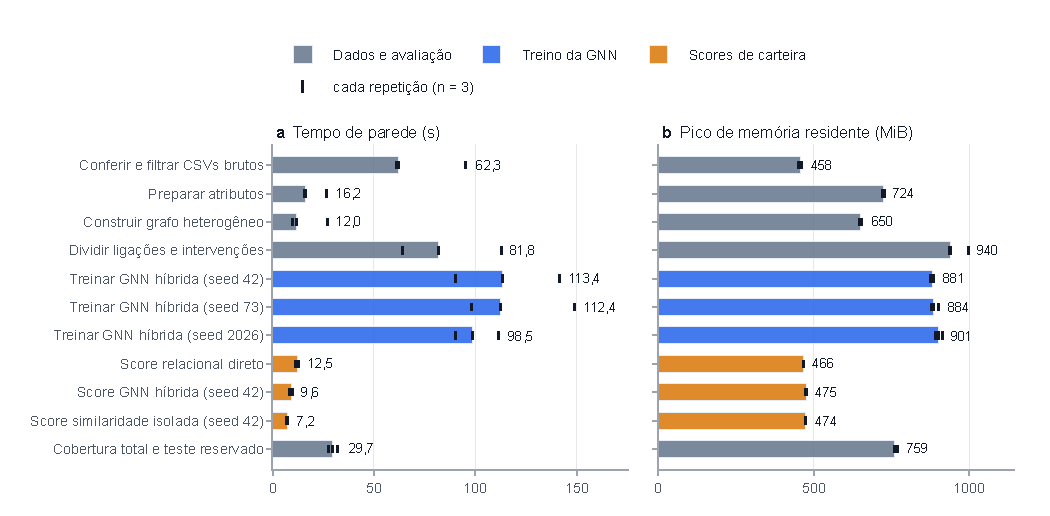
\includegraphics[width=\textwidth]{S4_tempos_memoria.pdf}
\caption{Custo por etapa do pipeline do dia real: barra = mediana de 3 repetições; traços = cada repetição (a primeira inclui cache frio). Pipeline completo: mediana de 8,7 min. Máquina: 13th Gen Intel(R) Core(TM) i3-1315U, 8 núcleos lógicos, 3,7 GiB, 2 threads por processo.}
\label{fig:s4}
\end{figure*}

% Alternativa: ROC e precisão-revocação lado a lado. Cada uma fica com 75% do tamanho desenhado
% (texto de cerca de 6 pt); prefira as figuras separadas acima se o periódico exigir 7 pt.
% \begin{figure*}[htbp]\centering
% 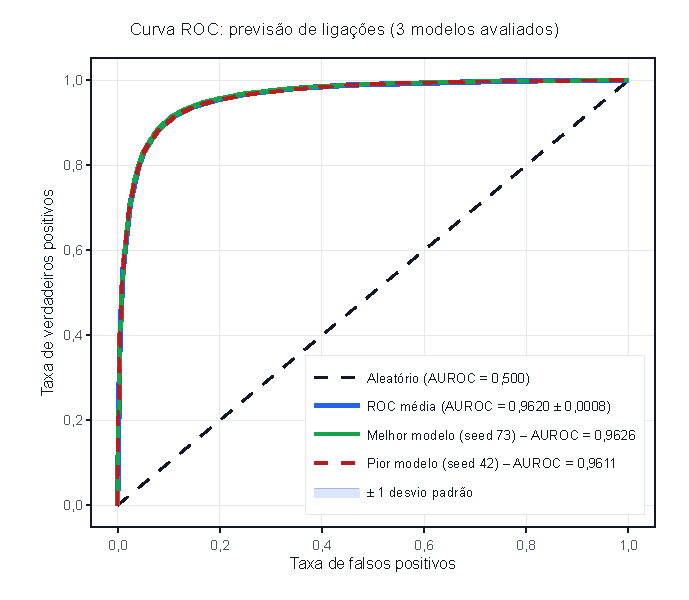
\includegraphics[width=0.49\textwidth]{G3_curva_roc.pdf}\hfill
% 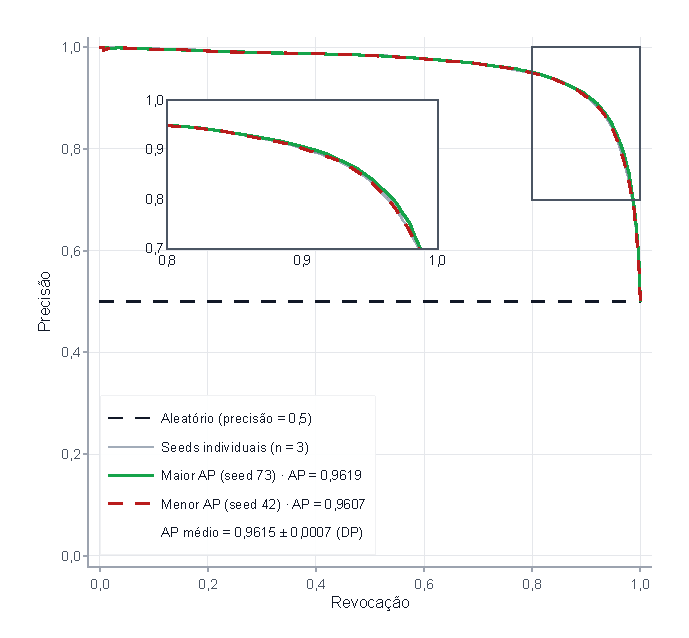
\includegraphics[width=0.49\textwidth]{S2_precisao_revocacao.pdf}
% \caption{(a) Curva ROC e (b) curva precisão-revocação das ligações reservadas.}
% \label{fig:roc-pr}
% \end{figure*}
